\subsection*{Převoz tyčí aneb reklama na Boba}
\label{sub:převoz_tyčí_aneb_reklama_na_Boba}

Zajištění tábora je po všech stránkách zajímavá a občas dost náročná záležitost, která se skládá z mnoha dílčích úkolů. Patří mezi ně hledání tábořiště, obvolávání a navštěvování vlastníků, plánování programů a mnoho dalších nutností. Jak už z názvu vyplývá, rád bych vám představil letošní úspěšný převoz.

Vše začíná na Kačerově, kde se scházíme v pátek v podvečer. Vyrážíme ve složení já(Humr a auto), Hafík, Koala a Terka . Dohoda s Bobem zní, že se potkáme s jeho tranzitem na kopci nad tábořištěm Hanyetu u Syrova. Vzhledem k očekávané situaci na dálnici (zprávami zrovna běžely hrůzné zkazky o ucpané D1) se rozhodujeme pro cestu přes Benešov a Vlašim. Cesta z Prahy, která by normálně měla trvat okolo 1 hodiny po dálnici se tak měla o půlhodinky prodloužit. Nápad jet přes Benešov má bohužel víc lidí, takže nakonec dorážíme na místo s 1,5hodinovým zpožděním. Bob se prozíravě rozhodl ignorovat fake news a přijíždí i s vozejkem po dálnici, takže si stíhá užít pěkný západ slunce a začít s taháním týpiovek. Tyče zbyly na tábořišti po zimních týpkařích – šlo jen o jedno týpí – zbytek je uložen na pile u Jiřiček. Za večer stihneme jakž takž vytahat tyče nahoru k autu – kopec bychom nevyjeli – a utábořit se na louce u Jiřiček. Večer se vyrábí večeře ze všech možných zbytků, kombinace nudlí, tortill, Terčina salátu(polníček?) a konzerv je lahodná.



\begin{center}

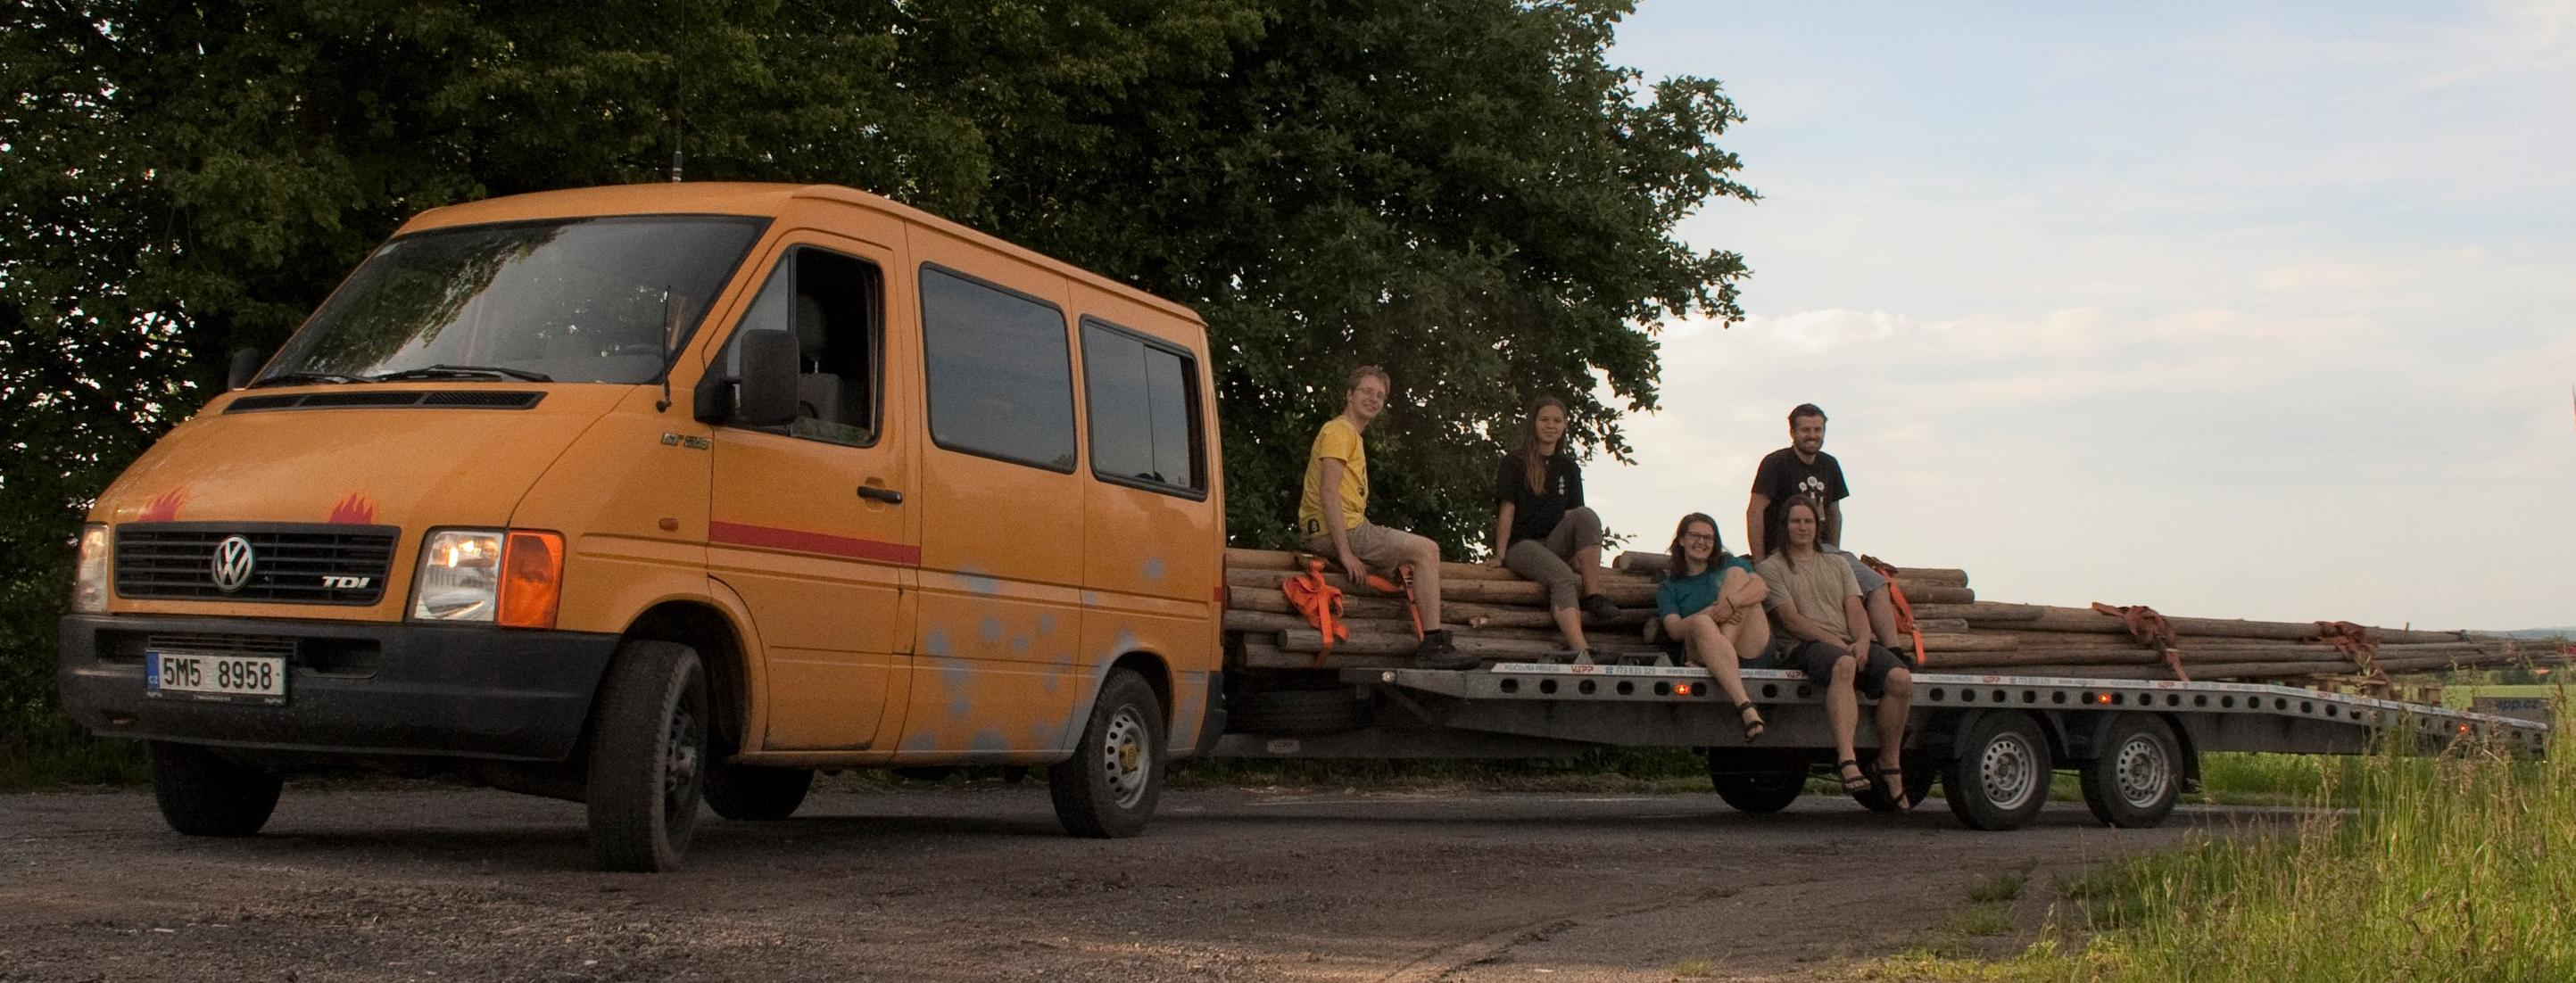
\includegraphics[width=12cm]{img/udo_clanky/Prevoz_tyci_2019_010.jpg}
\end{center}

Vstáváme brzy, abychom začali co nejdříve, čeká nás totiž převoz asi 150 kousků do 100 kilometrů vzdálené Vráže. Dle map bude cesta trvat 1,5 hodiny a nejsme si jisti, kolik tyčí zvládneme převézt v jedné várce. Každopádně, doufáme, že se nám podaří vše odvézt během dne, abychom byli večer doma (bláhové?).

Tyčí je mnoho, počítání náročné, 1.várka nám zabrala asi hodinu a čouhá metr a půl přes vozejk (většina tyčí má okolo 9m a více), snad tomu aspoň trochu pomůže červený praporek. Jedou obě vozidla – já s Koalou a Hafíkem se stavíme koupit oběd a potenciální večeři, a Bob s Terkou míří rovnou na tábořiště. Sraz máme ve Vráži u kapličky, s obědem i lahodnými zbytky od večeře čekáme na tyče. Voláme s tranzitem a zjišťujeme, že to vzali přes vesnici, ze které nevede most na druhý břeh Vltavy a teď musí vycouvat zpět na hlavní silnici. Nakonec doráží s mírným zpožděním, vykládáme tyče, necháváme doprovodné vozidlo ve Vráži a jedeme si pro další várku. Cestu si krátíme přednáškami z historie, recitací klasické arabské poezie, vyprávěním příběhů z dávných dob uďovství a debatováním o tématech, které si už nepamatuji, ale pamatuji si, že se o nich velmi živě debatovalo… Jo, a je pekelné vedro. 

Druhá várka nám jde od ruky a vypadá to, že bude náš tyčový park naložen, ale nakonec ještě asi 30 tyčí zbude. Pár tyčí pro jistotu seřízneme, naobědváme se a hurá směr Vráž. Témata pomalu dochází, spánek přichází. Bob naštěstí nespí a řídí. Poslední várku už nějak dotlačíme na vozík, vyfotíme se a odvezeme se. Jsme všichni mrtví a nechápeme, že Bob ještě zvládá řídit. Nu, je to Bob. Končíme v půl osmé po 12 hodinách převážení, nakládání a vykládání. Jdeme se ještě projít po Anpetu tábořišti, kde je všude vysoká tráva, takže se následně vracíme řádně oklíšťováni.
Nakonec nás čeká cesta do Prahy, během které posloucháme klasickou hudbu. 

Během převozu bylo celkem spáleno 90,3 litrů nafty a ujeto 832 km = průměrná spotřeba 10,85l/100km. Statistika namožených svalů a rozsezených zadků není k dispozici.

\podpis{Humr}



\subsection*{Nejlepší uďovský zážitek na táboře}
\label{sub:nejlepší_uďovský_zážitek_na_táboře}

Bohužel tento text vzniká přesně 131 dní po konci tábora, což znamená, že zážitky již v paměti nejsou tak živé. Nicméně, sepíšu alespoň sled výrazných událostí, které mě na táboře ovlivnily, a které přece jen ještě v paměti zůstávají.

Nakládáme materiál pro oba tábory náhodně do tranzitů, celý tábor si vozíme věci z jednoho tábořiště do druhého, Příšery si postupně kopají bazény v lese místo later(je tam fakt hodně vody), Urzoni jsou na stavebce, stavíme týpko na 4x, Špuntí šmouloprogram má úspěch, koupeme se o půlnoci v rybníce, král pirátů byl oběšen, Pískleti spadla sekera na hlavu, oholil jsem si vousy a nechal si jen velmi slušivý knír, dostali jsme kurděje a celý den se jí jen zelenina, Urzoni propíchli týpko chlopňovkou, Kámen kamení, během manévrů jachtíme v bezvětří na Orlíku, pozorujeme hvězdy, Jula přepadá tábor, Míček naučila papouška Kukumbrie novým hláškám, přeučujeme papouška na jiné hlášky, není sauna, Karkulka si zabodla dřevo do nohy, jedeme se koupat do Vltavy, holky smaží šílené množství řízků, poslední 2 dny tábora jíme jen řízky, šílené balení/vybalování a návrat z tábora, v Praze je maraton. 

\begin{center}

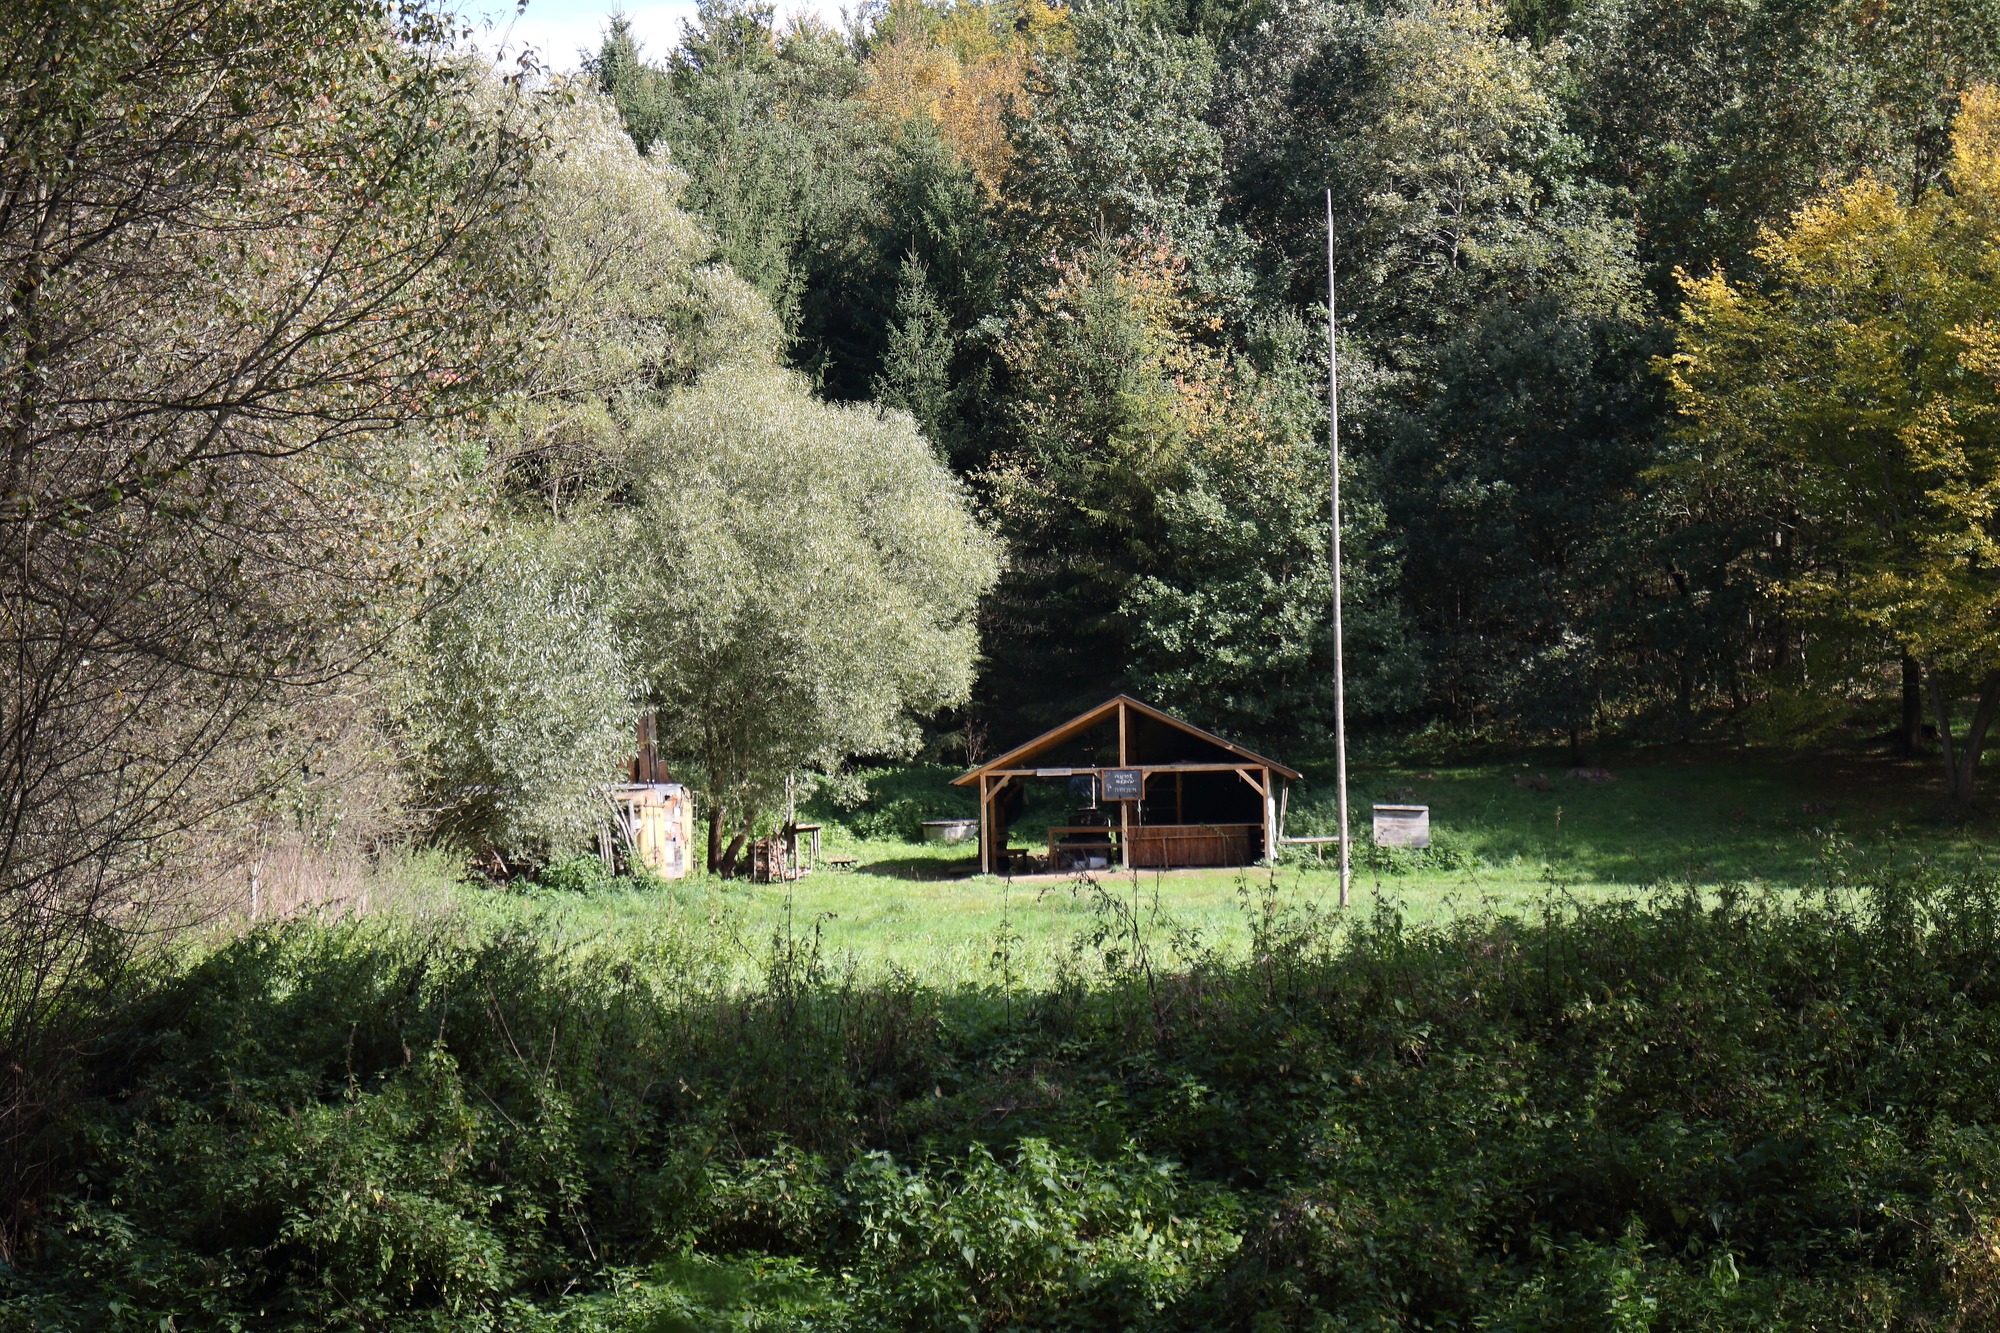
\includegraphics[width=10.2cm]{img/udo_clanky/hledanitaboriste.JPG}

\end{center}

\podpis{Humr}

\clearpage
